\documentclass[10pt,twocolumn]{article}

% ======================================================================
% PACKAGES
% ======================================================================
\usepackage[a4paper,top=0.62in,bottom=0.68in,left=0.62in,right=0.62in]{geometry}
\usepackage[T1]{fontenc}
\usepackage[utf8]{inputenc}
\usepackage{lmodern}
\usepackage{microtype}
\usepackage{amsmath}
\usepackage{amssymb}
\usepackage{mathtools}
\usepackage{booktabs}
\usepackage{multirow}
\usepackage{array}
\usepackage{tabularx}
\usepackage{makecell}
\usepackage{graphicx}
\usepackage{caption}
\usepackage{subcaption}
\usepackage{xcolor}
\usepackage{colortbl}
\usepackage{tikz}
\usetikzlibrary{arrows.meta,positioning,calc,fit,backgrounds,shapes.geometric}
\usepackage{pgfplots}
\pgfplotsset{compat=1.18}
\usepackage[most]{tcolorbox}
\usepackage{algorithm}
\usepackage{algpseudocode}
\usepackage{enumitem}
\usepackage[numbers,sort&compress]{natbib}
\usepackage{hyperref}
\usepackage[nameinlink,noabbrev]{cleveref}
\usepackage{balance}

% ======================================================================
% COLORS
% ======================================================================
\definecolor{CuraGreen}{HTML}{087F5B}
\definecolor{CuraDark}{HTML}{065F46}
\definecolor{CuraLight}{HTML}{ECFDF5}
\definecolor{AnnBlue}{HTML}{2563EB}
\definecolor{AnnLight}{HTML}{EFF6FF}
\definecolor{RiskRed}{HTML}{DC2626}
\definecolor{RiskLight}{HTML}{FEF2F2}
\definecolor{Gold}{HTML}{D97706}
\definecolor{GoldLight}{HTML}{FFFBEB}
\definecolor{Purple}{HTML}{7C3AED}
\definecolor{PurpleLight}{HTML}{F5F3FF}
\definecolor{Slate}{HTML}{334155}
\definecolor{MidGray}{HTML}{64748B}
\definecolor{VeryLightGray}{HTML}{F8FAFC}

% ======================================================================
% LINKS AND PAGE QUALITY
% ======================================================================
\hypersetup{colorlinks=true,linkcolor=CuraDark,citecolor=AnnBlue,urlcolor=AnnBlue,pdftitle={Beyond Recall: CURA -- Calibrated Utility-Risk Allocation},pdfauthor={Hrithik Sharma}}
\raggedbottom
\setlength{\columnsep}{0.27in}
\setlength{\parindent}{0pt}
\setlength{\parskip}{3pt}
\setlength{\emergencystretch}{3em}
\hfuzz=1pt
\renewcommand{\arraystretch}{1.10}
\captionsetup{font=small,labelfont=bf,skip=5pt}
\setlist[itemize]{leftmargin=14pt,itemsep=1.5pt,parsep=0pt,topsep=3pt}
\setlist[enumerate]{leftmargin=17pt,itemsep=2pt,parsep=0pt,topsep=3pt}

% ======================================================================
% COMMANDS
% ======================================================================
\newcommand{\cura}{CURA}
\newcommand{\ef}{\texttt{efSearch}}
\newcommand{\ndcg}{nDCG@10}
\newcommand{\annrec}{ANN Recall@10}
\newcommand{\deltandcg}{\Delta\mathrm{nDCG}@10}

% ======================================================================
% TIKZ STYLES -- NO BLANK LINES INSIDE THIS BLOCK
% ======================================================================
\tikzset{basebox/.style={rectangle,rounded corners=4pt,very thick,align=center,minimum height=0.85cm,font=\small},bluebox/.style={basebox,draw=AnnBlue,fill=AnnLight},greenbox/.style={basebox,draw=CuraGreen,fill=CuraLight},redbox/.style={basebox,draw=RiskRed,fill=RiskLight},goldbox/.style={basebox,draw=Gold,fill=GoldLight},purplebox/.style={basebox,draw=Purple,fill=PurpleLight},flow/.style={-{Latex[length=2.4mm]},thick,draw=Slate},greenflow/.style={-{Latex[length=2.4mm]},thick,draw=CuraGreen}}

% ======================================================================
% DOCUMENT
% ======================================================================
\begin{document}

% ======================================================================
% FULL-WIDTH TITLE + ABSTRACT
% ======================================================================
\twocolumn[
\begin{@twocolumnfalse}
\begin{center}
{\LARGE\bfseries Beyond Recall: CURA\par}
\vspace{0.12cm}
{\large Calibrated Utility-Risk Allocation for\\Query-Specific Approximate Nearest Neighbor Search\par}
\vspace{0.28cm}
{\normalsize\textbf{Hrithik Sharma}\par}
\vspace{0.05cm}
{\small Indian Institute of Technology Delhi\par}
{\small COL764 -- Information Retrieval and Web Search\par}
\vspace{0.22cm}
\end{center}
\noindent\rule{\textwidth}{0.65pt}
\vspace{0.10cm}
\begin{minipage}{0.97\textwidth}
\small
\textbf{Abstract.}
Approximate nearest neighbor (ANN) retrieval systems commonly allocate search effort according to ANN-centric criteria such as neighbor recall. However, recovering the exact nearest-neighbor set may require more computation than is necessary to preserve downstream information-retrieval quality.

We investigate this mismatch for HNSW retrieval and introduce \textbf{\cura{} (Calibrated Utility-Risk Allocation)}, a query-specific search-budget controller that predicts the probability that a candidate search budget will cause downstream nDCG@10 degradation greater than a predefined tolerance. Rather than optimizing exact-neighbor recovery directly, \cura{} selects the smallest search budget whose calibrated probability of unacceptable downstream degradation is sufficiently low.

We evaluate the method on a controlled million-scale MS MARCO experiment containing \textbf{1,000,629 passages}. MS MARCO development queries are partitioned into query-disjoint training, calibration, and held-out test sets, while TREC-DL-2019 is reserved for out-of-distribution evaluation.

On held-out MS MARCO, \cura{}-Full maintains a \textbf{1.0\% downstream utility violation rate under a 5\% risk target} while reducing realized HNSW distance computations from \textbf{3431.77 to 2727.97 per query}, corresponding to a \textbf{20.5\% reduction relative to fixed-budget retrieval}. The paired mean reduction is \textbf{703.81 distance computations/query}, with a bootstrap 95\% confidence interval of \textbf{[401.43, 984.11]} and paired-randomization \textbf{$p\approx5\times10^{-5}$}.

Compared with an ANN-risk adaptive controller, \cura{} requires approximately \textbf{30.6\% less realized search work}. Ablations show that cheap partial-search-state features are essential: a query-only variant requires substantially more computation. A second BEIR FiQA financial-domain experiment finds that a reduced-feature controller fitted separately on FiQA requires 75.3\% more work than calibrated fixed HNSW despite identical observed violations. Fifty actual low-budget FiQA failures have been selected for human review, which is not yet complete.

These results support treating ANN recall and downstream retrieval utility as related but non-interchangeable objectives for adaptive retrieval.
\end{minipage}
\vspace{0.10cm}
\noindent\rule{\textwidth}{0.65pt}
\vspace{0.35cm}
\end{@twocolumnfalse}
]

% ======================================================================
% 1 INTRODUCTION
% ======================================================================
\section{Introduction}
\label{sec:introduction}
Dense retrieval systems map queries and documents into a vector space and retrieve nearby vectors using approximate nearest neighbor search. At large collection sizes, exhaustive comparison against every document embedding is expensive, motivating efficient ANN indexes such as HNSW~\citep{malkov2020hnsw}, FAISS~\citep{johnson2017faiss}, DiskANN~\citep{subramanya2019diskann}, and ScaNN~\citep{guo2020scann}.

HNSW exposes a runtime exploration parameter, commonly called \ef{}, that directly affects the effectiveness--efficiency trade-off. Larger values usually increase exact-neighbor recovery, but also increase graph exploration, distance computations, and latency.

A conventional system therefore asks:
\begin{quote}
\emph{How much search effort is required to achieve a desired ANN recall?}
\end{quote}

For an information-retrieval application, however, exact vector-neighbor recovery is an intermediate objective rather than the final goal. The system ultimately cares whether relevant passages remain highly ranked, typically measured with metrics such as nDCG~\citep{jarvelin2002cg}.

A missed exact neighbor can be harmless when an approximately equivalent relevant passage replaces it. Conversely, high ANN recall does not guarantee preservation of the specific documents that matter most to the downstream ranking.

\begin{tcolorbox}[colback=GoldLight,colframe=Gold,boxrule=0.8pt,arc=3pt,left=5pt,right=5pt,top=4pt,bottom=4pt]
\small
\textbf{Research Question.}
Can ANN computation be allocated according to the predicted probability of harming downstream retrieval quality rather than according to exact-neighbor recovery alone?
\end{tcolorbox}

% ======================================================================
% RESEARCH APPROACH DIAGRAM
% ======================================================================
\begin{figure*}[!t]
\centering
\resizebox{0.96\textwidth}{!}{%
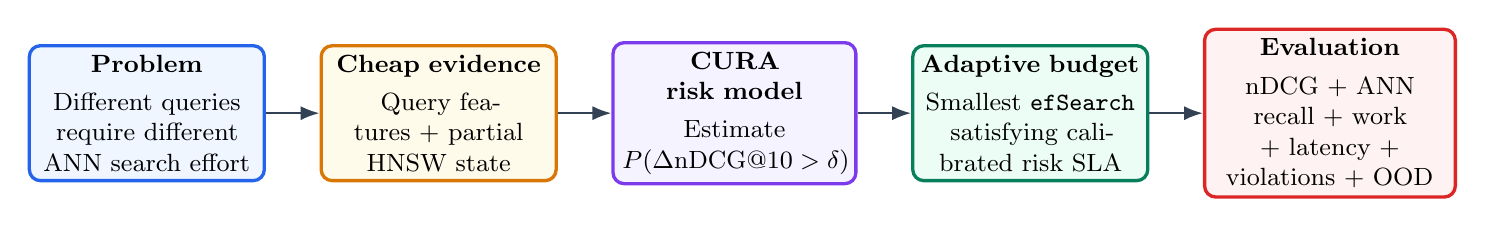
\begin{tikzpicture}[node distance=0.68cm]
\node[bluebox,text width=2.75cm] (problem) {\textbf{Problem}\\[1mm]Different queries require different ANN search effort};
\node[goldbox,text width=2.75cm,right=of problem] (signals) {\textbf{Cheap evidence}\\[1mm]Query features + partial HNSW state};
\node[purplebox,text width=2.85cm,right=of signals] (risk) {\textbf{CURA risk model}\\[1mm]Estimate $P(\deltandcg>\delta)$};
\node[greenbox,text width=2.75cm,right=of risk] (budget) {\textbf{Adaptive budget}\\[1mm]Smallest \ef{} satisfying calibrated risk SLA};
\node[redbox,text width=2.95cm,right=of budget] (evaluation) {\textbf{Evaluation}\\[1mm]nDCG + ANN recall + work + latency + violations + OOD};
\draw[flow] (problem) -- (signals);
\draw[flow] (signals) -- (risk);
\draw[flow] (risk) -- (budget);
\draw[flow] (budget) -- (evaluation);
\end{tikzpicture}%
}
\vspace{0.10cm}
\caption{\textbf{Research approach.} The query-specific ANN budgeting problem is formulated as calibrated downstream-risk allocation. The controller uses inexpensive query and partial-search information and is evaluated jointly on retrieval effectiveness, ANN quality, efficiency, calibration, and distribution shift.}
\label{fig:approach}
\end{figure*}

\subsection{Research Scope}
The project studies \textbf{query-specific ANN search-budget allocation}. Instead of assigning every query a single global HNSW configuration, the goal is to determine how much graph exploration each individual query needs.

The experimental design follows four principles.
\begin{enumerate}
\item \textbf{Query-specific budgeting.} The controller selects a different \ef{} for different queries.
\item \textbf{Cheap decision signals.} The controller uses query features and inexpensive partial-search information rather than exact search or relevance judgments at inference time.
\item \textbf{Calibrated constraint satisfaction.} Budget selection is based on an estimated probability of downstream ranking failure.
\item \textbf{Joint effectiveness--efficiency evaluation.} ANN quality and end-to-end IR effectiveness are evaluated together with distance computations, latency, calibration, and violation rates.
\end{enumerate}

\subsection{Hypothesis}
\begin{tcolorbox}[colback=CuraLight,colframe=CuraGreen,boxrule=0.8pt,arc=3pt,left=5pt,right=5pt,top=4pt,bottom=4pt]
\small
\textbf{H1.} At a matched downstream-quality risk target, a query-specific policy using query and partial-search-state features can require significantly fewer HNSW distance computations than globally fixed search.
\end{tcolorbox}

The backoff hypothesis is that even if a learned adaptive controller does not yield consistent savings, ANN-safe and downstream-IR-safe search budgets will exhibit systematic query-dependent differences that can be explained by query hardness and evaluation regime.

\subsection{Contributions}
This work makes five main contributions.
\begin{enumerate}
\item \textbf{ANN-versus-IR budget analysis.} We quantify query-level differences between the minimum HNSW budget required for ANN reconstruction and the budget required to preserve downstream ranking quality.
\item \textbf{Calibrated utility-risk allocation.} We introduce \cura{}, which models
\[
P(\deltandcg>\delta\mid q,S,e)
\]
instead of directly predicting ANN recall.
\item \textbf{Leakage-safe million-scale evaluation.} Training, calibration, and testing are separated by query, with TREC-DL-2019 held out for OOD evaluation.
\item \textbf{Substantive ablations.} We evaluate fixed search, ANN-risk adaptation, query-only \cura{}, full \cura{}, a Patience-inspired stability baseline, and oracle references.
\item \textbf{Statistical and qualitative validation.} We report paired randomization tests, bootstrap confidence intervals, probability calibration, hardness analysis, and a 50-case evidence worksheet awaiting complete human verification.
\end{enumerate}

% ======================================================================
% 2 RELATED WORK
% ======================================================================
\section{Related Work}
\label{sec:related}
\subsection{Approximate Nearest Neighbor Search}
HNSW constructs a hierarchical proximity graph for efficient approximate nearest-neighbor retrieval~\citep{malkov2020hnsw}. FAISS provides widely used exact and approximate vector-search implementations~\citep{johnson2017faiss}. Other scalable systems include DiskANN~\citep{subramanya2019diskann} and ScaNN~\citep{guo2020scann}.

ANN-Benchmarks emphasizes evaluation across the accuracy--performance frontier rather than at only one operating point~\citep{aumuller2020ann}.

\subsection{Accelerating Dense Retrieval}
LADR combines lexical retrieval signals with dense retrieval to reduce dense-search cost~\citep{kulkarni2023ladr}. Zhang et al. propose the Hybrid Inverted Index, combining embedding clusters and lexical signals to accelerate dense retrieval~\citep{zhang2023hybrid}. Busolin et al. study early-exit strategies for approximate $k$-NN search in dense retrieval and demonstrate substantial efficiency gains~\citep{busolin2024early}.

\subsection{Adaptive HNSW Search}
Zhang and Miller propose distribution-aware adaptive HNSW exploration, dynamically configuring the exploration factor according to query and distribution characteristics~\citep{zhang2026adaptive}. Patience in Proximity introduces an early-termination mechanism for HNSW graph traversal~\citep{teofili2025patience}. DARTH addresses declarative recall targets through learned early termination for ANN search~\citep{chatzakis2026darth}. Terminus introduces rank-aware early termination for vector search~\citep{lu2026terminus}.

\subsection{Positioning of CURA}
The distinguishing feature of \cura{} is not merely predicting \ef{}. Instead, \cura{} treats a \textbf{qrel-derived downstream ranking failure} as the supervised event and estimates a calibrated probability that a candidate budget violates that downstream quality requirement.

\begin{tcolorbox}[colback=PurpleLight,colframe=Purple,title=\textbf{Novelty of CURA},fonttitle=\small,boxrule=0.8pt,arc=3pt]
\small
\cura{} combines:
\begin{enumerate}
\item a downstream loss event, $\deltandcg>\delta$;
\item query and cheap partial-search-state features;
\item probability calibration;
\item explicit downstream-risk SLA selection;
\item held-out and distribution-shift evaluation;
\item realized adaptive-search cost accounting.
\end{enumerate}
\end{tcolorbox}

\begin{table*}[!t]
\centering
\caption{\textbf{Positioning relative to closely related ANN-efficiency approaches.} The table distinguishes the quantity used to decide whether additional search is required.}
\label{tab:novelty}
\resizebox{0.95\textwidth}{!}{%
\begin{tabular}{lllll}
\toprule
\textbf{Method} & \textbf{Adaptive} & \textbf{Decision signal} & \textbf{Primary objective} & \textbf{Calibrated downstream SLA} \\
\midrule
Fixed HNSW & No & None & Global search budget & No \\
Busolin et al.~\citep{busolin2024early} & Yes & Search progress & Early exit & No \\
Patience~\citep{teofili2025patience} & Yes & HNSW traversal progress & Early termination & No \\
Ada-ef~\citep{zhang2026adaptive} & Yes & Distribution statistics & Target ANN recall & No \\
DARTH~\citep{chatzakis2026darth} & Yes & ANN search state & Target ANN recall & No \\
Terminus~\citep{lu2026terminus} & Yes & Rank-aware utility & Rank-weighted search utility & No \\
\rowcolor{CuraLight}
\textbf{CURA} & \textbf{Yes} & \textbf{Query + partial-search state} & \textbf{$P(\deltandcg>\delta)$} & \textbf{Yes} \\
\bottomrule
\end{tabular}%
}
\end{table*}

% ======================================================================
% 3 PROBLEM FORMULATION
% ======================================================================
\section{Problem Formulation}
\label{sec:problem}
Let $q$ denote a query and let $e$ denote a candidate HNSW search budget. Let $U^\star(q)$ be the downstream effectiveness obtained by exact vector retrieval and $U(q,e)$ the effectiveness obtained using HNSW at budget $e$. For the primary experiment,
\[
U=\mathrm{nDCG}@10.
\]
We define downstream utility loss as
\begin{equation}
\Delta U(q,e)=U^\star(q)-U(q,e).
\label{eq:utilityloss}
\end{equation}
A query-budget pair is considered IR-unsafe when
\begin{equation}
\Delta U(q,e)>\delta,\qquad \delta=0.025.
\label{eq:irunsafe}
\end{equation}
For comparison, an ANN-centric pair is unsafe when
\begin{equation}
\mathrm{Recall}@10(q,e)<0.90.
\label{eq:annunsafe}
\end{equation}
\cura{} estimates
\begin{equation}
r(q,e)=P\left(\Delta U(q,e)>\delta\mid q,S_q,e\right),
\label{eq:risk}
\end{equation}
where $S_q$ contains deployable partial-search-state information. The desired policy is
\begin{equation}
e^\star(q)=\min_{e\in\mathcal E}\{e:r(q,e)\le\tau\},
\label{eq:budgetselection}
\end{equation}
where $\tau$ is chosen only using the calibration split.

% ======================================================================
% 4 METHOD
% ======================================================================
\section{CURA}
\label{sec:method}
\subsection{Feature Design}
Only inference-time information is used.

\paragraph{Query features.}
The query-only component uses character count, token count, average token length, digit and question-mark indicators, PCA components of the query embedding, candidate \ef{}, and budget transformations.

\paragraph{Partial-search features.}
A cheap HNSW probe at $\ef=10$ produces top candidate scores, score mean and standard deviation, several score margins, HNSW distance computations, and graph hops. These signals capture local score geometry and search-state uncertainty.

\subsection{Risk Predictor}
We train a histogram gradient-boosted classifier on query-budget pairs. The target is
\[
y_{\mathrm{IR}}(q,e)=\mathbb{1}[\Delta U(q,e)>\delta].
\]
Class-balanced weighting compensates for the small unsafe class.

\subsection{Probability Calibration}
Raw classifier scores are calibrated with isotonic regression on calibration queries. Calibration is important because \cura{} makes an explicit predicted-risk decision~\citep{guo2017calibration}. The current procedure can reuse calibration queries for probability fitting and policy selection; a separate operating-point split is preferable for stronger claims.

\subsection{Operating Threshold}
For candidate thresholds, we select one budget for every calibration query and compute the empirical downstream violation rate. A conservative 95\% Wilson upper confidence bound is then computed. Among settings satisfying the target risk constraint, we select the one with minimum mean search effort.

\begin{algorithm}[!t]
\caption{\cura{} inference}
\label{alg:cura}
\begin{algorithmic}[1]
\Require Query $q$, candidate budgets $\mathcal E$, calibrated model $R$, threshold $\tau$
\State Extract query features $x_q$
\State Run inexpensive HNSW probe at $e_0=10$
\State Extract partial-search state $S_q$
\For{$e\in\mathcal E$ in increasing order}
\State $p_e\gets R(x_q,S_q,e)$
\If{$p_e\le\tau$}
\State \Return $e$
\EndIf
\EndFor
\State \Return $\max(\mathcal E)$
\end{algorithmic}
\end{algorithm}

\begin{figure*}[!t]
\centering
\resizebox{0.94\textwidth}{!}{%
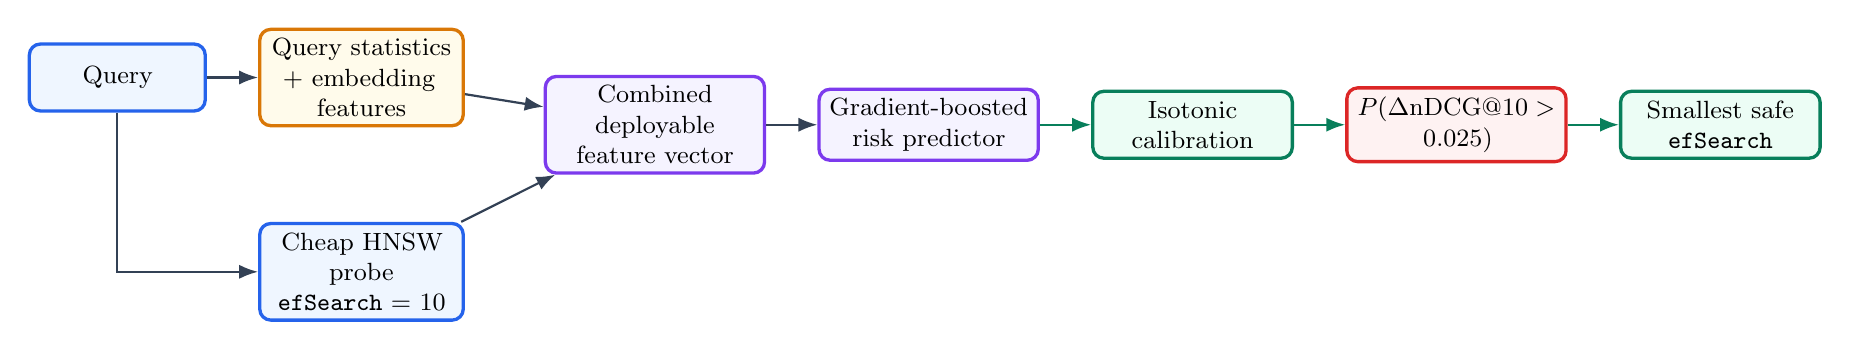
\begin{tikzpicture}[node distance=0.65cm]
\node[bluebox,text width=2.0cm] (query) {Query};
\node[goldbox,text width=2.35cm,right=of query] (embedding) {Query statistics + embedding features};
\node[bluebox,text width=2.35cm,below=1.20cm of embedding] (probe) {Cheap HNSW probe\\$\ef=10$};
\node[purplebox,text width=2.55cm,right=1.00cm of embedding,yshift=-0.60cm] (features) {Combined deployable feature vector};
\node[purplebox,text width=2.55cm,right=of features] (model) {Gradient-boosted risk predictor};
\node[greenbox,text width=2.30cm,right=of model] (cal) {Isotonic calibration};
\node[redbox,text width=2.55cm,right=of cal] (risk) {$P(\Delta\mathrm{nDCG}@10>0.025)$};
\node[greenbox,text width=2.30cm,right=of risk] (selection) {Smallest safe \ef{}};
\draw[flow] (query) -- (embedding);
\draw[flow] (query.south) |- (probe.west);
\draw[flow] (embedding) -- (features);
\draw[flow] (probe) -- (features);
\draw[flow] (features) -- (model);
\draw[greenflow] (model) -- (cal);
\draw[greenflow] (cal) -- (risk);
\draw[greenflow] (risk) -- (selection);
\end{tikzpicture}%
}
\caption{\textbf{CURA architecture.} The controller combines query features with an inexpensive partial HNSW probe, predicts downstream ranking-failure risk, calibrates the probability, and selects the smallest budget satisfying the quality-risk constraint.}
\label{fig:curaarchitecture}
\end{figure*}

% ======================================================================
% 5 EXPERIMENTAL SETUP
% ======================================================================
\section{Experimental Setup}
\label{sec:setup}
\subsection{Datasets}
MS MARCO provides a large passage-retrieval benchmark built from real search queries~\citep{bajaj2016msmarco}. The complete passage collection contains approximately 8.8 million passages. Given the available local compute budget, our primary experiment constructs a deterministic controlled collection containing
\[
\boxed{1,000,629\text{ passages}.}
\]
All judged passages for selected evaluation queries are guaranteed to appear in the collection. Remaining background passages are deterministically sampled.

The experiment includes 1,000 MS MARCO development queries and 43 TREC-DL-2019 queries. TREC-DL-2019 contains deeply judged passage-ranking queries and is used as the distribution-shift evaluation set~\citep{craswell2020trecdl}.

\paragraph{Preliminary SciFact pilot.}
Before the large MS MARCO experiment, a small SciFact pilot was used to validate the experimental pipeline. That pilot suggested that downstream-safe and ANN-safe budget requirements could differ, but SciFact was too small to support strong HNSW systems conclusions. The final analysis therefore scales the experiment to MS MARCO rather than treating the SciFact result as primary evidence.

\paragraph{Financial-domain experiment.}
We also investigate BEIR FiQA with 57,638 documents and 648 published test queries in a budget sweep. A subsequent, separately fitted simplified controller uses 388 training queries, 129 calibration queries, and 131 locally held-out queries. This is exploratory because official test queries are reused for development; it is not zero-shot transfer of the MS MARCO CURA-Full model.

\subsection{Dense Encoder}
We use the fixed dense encoder \texttt{sentence-transformers/msmarco-MiniLM-L6-cos-v5}. The embedding dimension is $d=384$. All vectors are normalized and searched using inner product, corresponding to cosine similarity for normalized embeddings. The sentence-transformer architecture follows Reimers and Gurevych~\citep{reimers2019sbert}.

\subsection{Exact Reference}
Exact retrieval uses a FAISS IndexFlatIP reference index~\citep{johnson2017faiss}. This exact result serves as the vector-space reference when computing ANN recall and downstream degradation.

\subsection{HNSW Configuration}
Our HNSW configuration is
\[
M=32,\qquad \texttt{efConstruction}=200.
\]
For the main top-10 experiment,
\[
\mathcal E=\{10,16,24,32,48,64,96,128,192,256\}.
\]
For the top-100 validation,
\[
\mathcal E_{100}=\{100,150,200,300,400,600,800\}.
\]

\subsection{Query Splits}
MS MARCO development queries are divided by query ID into 60\% training, 20\% calibration, and 20\% held-out testing. All TREC-DL-2019 queries are excluded from training and calibration.

\begin{figure*}[!t]
\centering
\resizebox{0.95\textwidth}{!}{%
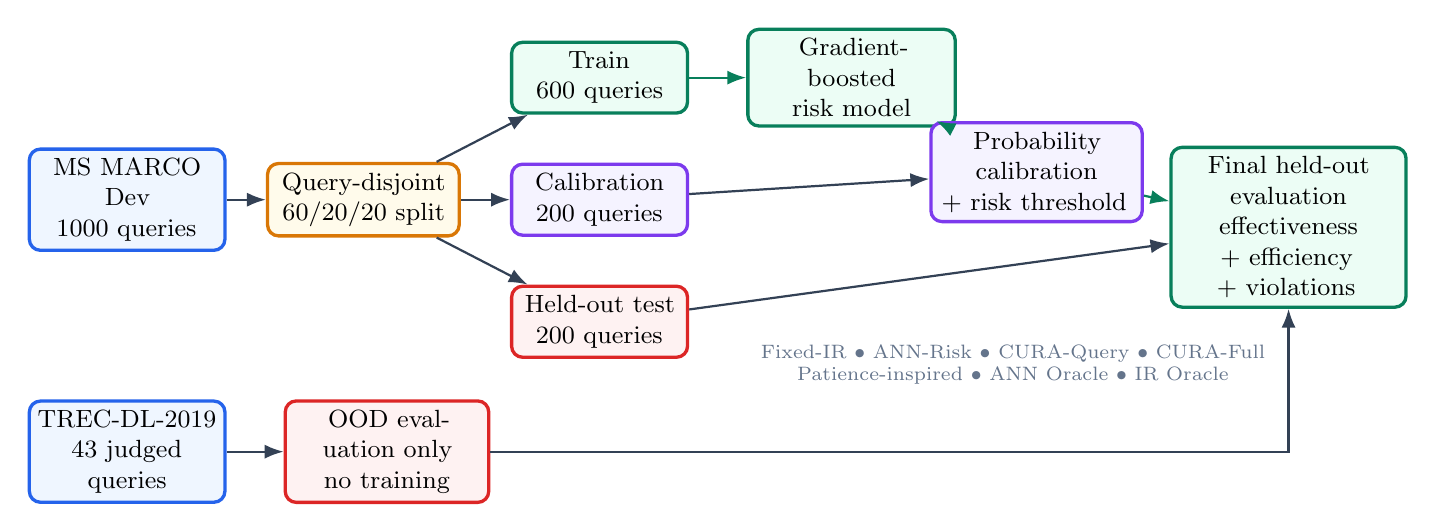
\begin{tikzpicture}[font=\small]
\node[bluebox,text width=2.25cm] (msmarco) at (0,0) {MS MARCO Dev\\1000 queries};
\node[goldbox,text width=2.20cm] (split) at (3.0,0) {Query-disjoint\\60/20/20 split};
\node[greenbox,text width=2.0cm] (train) at (6.0,1.55) {Train\\600 queries};
\node[purplebox,text width=2.0cm] (calibrationSet) at (6.0,0) {Calibration\\200 queries};
\node[redbox,text width=2.0cm] (test) at (6.0,-1.55) {Held-out test\\200 queries};
\node[greenbox,text width=2.40cm] (model) at (9.2,1.55) {Gradient-boosted\\risk model};
\node[purplebox,text width=2.45cm] (calibration) at (11.55,0.35) {Probability calibration\\+ risk threshold};
\node[greenbox,text width=2.75cm] (evaluation) at (14.75,-0.35) {Final held-out evaluation\\effectiveness + efficiency\\+ violations};
\node[bluebox,text width=2.25cm] (trec) at (0,-3.20) {TREC-DL-2019\\43 judged queries};
\node[redbox,text width=2.35cm] (ood) at (3.30,-3.20) {OOD evaluation only\\no training};
\draw[flow] (msmarco) -- (split);
\draw[flow] (split) -- (train);
\draw[flow] (split) -- (calibrationSet);
\draw[flow] (split) -- (test);
\draw[greenflow] (train) -- (model);
\draw[greenflow] (model) -- (calibration);
\draw[flow] (calibrationSet) -- (calibration);
\draw[greenflow] (calibration) -- (evaluation);
\draw[flow] (test) -- (evaluation);
\draw[flow] (trec) -- (ood);
\draw[flow] (ood.east) -| (evaluation.south);
\node[align=center,text=MidGray,font=\scriptsize] at (11.25,-2.10) {Fixed-IR $\bullet$ ANN-Risk $\bullet$ CURA-Query $\bullet$ CURA-Full\\Patience-inspired $\bullet$ ANN Oracle $\bullet$ IR Oracle};
\end{tikzpicture}%
}
\caption{\textbf{Leakage-safe evaluation protocol.} MS MARCO queries are separated before model fitting. Training queries fit the risk model, calibration queries determine probability calibration and the operating point, and held-out test queries are used only for final evaluation. TREC-DL-2019 is excluded from training and calibration.}
\label{fig:evaluation}
\end{figure*}

\subsection{Metrics}
Effectiveness measures include ANN Recall@10, nDCG@10, Recall@100, MRR@10, and downstream violation rate. Efficiency measures include HNSW distance computations, mean latency, p95 latency, selected \ef{}, and adaptive-controller overhead. Calibration metrics include Brier score, Expected Calibration Error (ECE), and ROC-AUC.

\subsection{Realized Adaptive Cost}
Adaptive systems require additional computation to decide when to stop. Therefore our primary cost measure is \textbf{realized HNSW distance computations}. For \cura{}-Full this includes the cheap $\ef=10$ probe and the selected search when a larger budget is required. For the stability baseline, realized work includes every search executed along the increasing budget ladder.

\subsection{Compute Budget}
The million-scale experiment is run using CPU-based FAISS search. Expensive preprocessing stages are cached. Observed one-time costs include approximately \textbf{3 h 39 min 50 s} for corpus encoding and \textbf{778.58 s} for HNSW construction.

\begin{tcolorbox}[colback=RiskLight,colframe=RiskRed,title=\textbf{Leakage Control},fonttitle=\small,boxrule=0.8pt]
\small
At inference time, \cura{} never observes relevance judgments, exact nearest-neighbor identities, ANN recall, exact nDCG, or downstream loss labels. These quantities are used only to construct supervised labels and evaluate the method. PCA is also fitted exclusively on training-query embeddings.
\end{tcolorbox}

% ======================================================================
% 6 ORACLE ANALYSIS
% ======================================================================
\section{ANN Recall versus Downstream Utility}
\label{sec:oracle}
Before fitting an adaptive controller, we ask whether ANN-safe and IR-safe queries actually require different search budgets.

At million scale, the mean top-10 ANN-safe oracle budget is approximately $21.39$, while the mean downstream nDCG-safe oracle budget is approximately $12.62$. This corresponds to roughly a
\[
\boxed{41.0\%}
\]
reduction in oracle budget.

Importantly, this is an \textbf{oracle opportunity rather than a deployable speedup}. The oracle knows the outcome at every budget.

\subsection{Domain-Specific Validation}
The effect is not equally strong under every relevance-judgment regime. In the earlier 200K analysis, MS MARCO development queries exhibit a large and statistically supported downstream-versus-ANN oracle gap, whereas TREC-DL-2019 exhibits a much weaker gap with insufficient evidence for the same phenomenon. This negative result prevents the stronger unsupported conclusion that downstream utility always requires less search effort.

% ======================================================================
% 7 MAIN RESULTS
% ======================================================================
\section{Main Results}
\label{sec:results}
The central question is whether the deployable \cura{} controller can convert oracle headroom into real search-work reductions without violating the downstream quality constraint.

\begin{tcolorbox}[colback=CuraLight,colframe=CuraGreen,title=\textbf{Primary Held-Out Result},fonttitle=\small,coltitle=CuraDark,boxrule=0.9pt,arc=3pt,left=5pt,right=5pt,top=4pt,bottom=4pt]
\small
On held-out MS MARCO, \textbf{\cura{}-Full} maintains a \textbf{1.0\% downstream violation rate} under the predefined \textbf{5\% risk SLA}, while reducing realized HNSW work from
\[
3431.77\quad\longrightarrow\quad2727.97
\]
distance computations per query. Thus \cura{} achieves a
\[
\boxed{\textbf{20.5\% reduction}}
\]
relative to fixed-budget retrieval.
\end{tcolorbox}

\begin{table*}[!t]
\centering
\caption{\textbf{Held-out MS MARCO results.} IR Viol. denotes the proportion of queries exceeding the predefined nDCG-loss tolerance. Search work includes adaptive overhead where applicable.}
\label{tab:mainresults}
\resizebox{0.96\textwidth}{!}{%
\begin{tabular}{lrrrrrrr}
\toprule
\textbf{Method} & \textbf{Mean ef} & \textbf{IR Viol.} & \textbf{ANN Viol.} & \textbf{Mean nDCG@10} & \textbf{Search Work} & \textbf{Work saving} & \textbf{Latency (ms)} \\
\midrule
Fixed-IR & 96.00 & 0.5\% & 3.5\% & 0.625260 & 3431.770 & 0.0\% & 0.8329 \\
ANN-Risk & 84.46 & 0.5\% & 1.5\% & 0.625260 & 3930.615 & $-14.5\%$ & 0.9580 \\
CURA-Query & 225.92 & 0.0\% & 2.0\% & 0.626970 & 7130.760 & $-107.8\%$ & 1.7156 \\
\rowcolor{CuraLight}
\textbf{CURA-Full} & \textbf{51.97} & \textbf{1.0\%} & 10.0\% & 0.623363 & \textbf{2727.965} & \textbf{20.5\%} & \textbf{0.6907} \\
Patience-Inspired & 62.32 & 0.5\% & 5.0\% & 0.625260 & 8413.945 & $-145.2\%$ & 2.1693 \\
\midrule
ANN-Oracle & 22.50 & 0.5\% & 1.0\% & 0.626896 & 1208.020 & 64.8\% & 0.3506 \\
IR-Oracle & 11.51 & 0.0\% & 29.0\% & 0.630348 & 779.835 & 77.3\% & 0.2697 \\
\bottomrule
\end{tabular}%
}
\end{table*}

\begin{figure*}[!t]
\centering
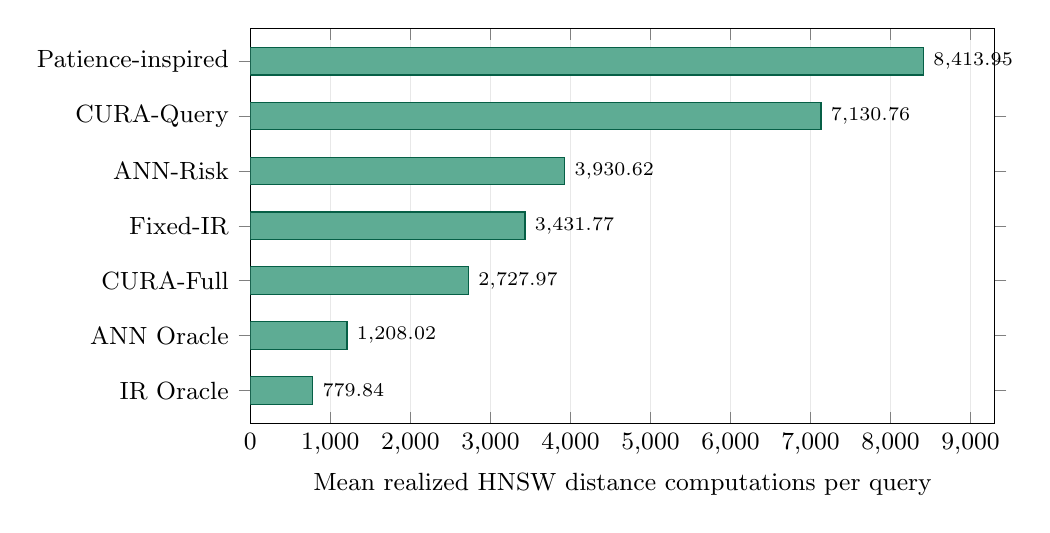
\begin{tikzpicture}
\begin{axis}[width=0.91\textwidth,height=6.6cm,xbar,bar width=10pt,xlabel={Mean realized HNSW distance computations per query},symbolic y coords={IR Oracle,ANN Oracle,CURA-Full,Fixed-IR,ANN-Risk,CURA-Query,Patience-inspired},ytick=data,xmin=0,xmax=9300,xmajorgrids=true,grid style={gray!18},axis line style={black},tick label style={font=\small,text=black},label style={font=\small,text=black},nodes near coords,nodes near coords align={horizontal},every node near coord/.append style={font=\scriptsize,text=black,anchor=west}]
\addplot[fill=CuraGreen!65,draw=CuraDark] coordinates {(779.84,IR Oracle) (1208.02,ANN Oracle) (2727.97,CURA-Full) (3431.77,Fixed-IR) (3930.62,ANN-Risk) (7130.76,CURA-Query) (8413.95,Patience-inspired)};
\end{axis}
\end{tikzpicture}
\caption{\textbf{Realized search work on held-out MS MARCO.} \cura{}-Full requires fewer HNSW distance computations than fixed search, ANN-risk adaptation, and the Patience-inspired stability baseline. The oracle methods quantify remaining theoretical headroom.}
\label{fig:searchwork}
\end{figure*}

\begin{figure*}[!t]
\centering
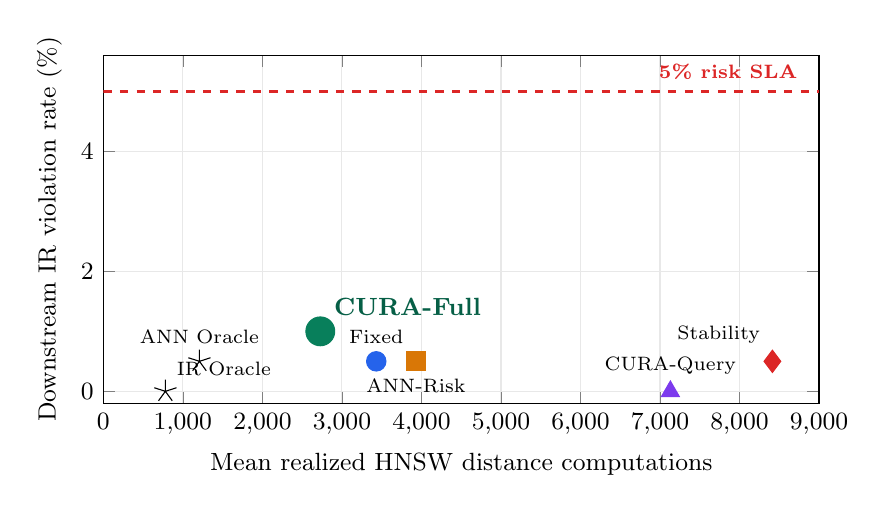
\begin{tikzpicture}
\begin{axis}[width=0.88\textwidth,height=6.0cm,xlabel={Mean realized HNSW distance computations},ylabel={Downstream IR violation rate (\%)},xmin=0,xmax=9000,ymin=-0.20,ymax=5.6,xmajorgrids=true,ymajorgrids=true,grid style={gray!18},axis line style={black},tick label style={font=\small,text=black},label style={font=\small,text=black}]
\addplot[RiskRed,dashed,very thick] coordinates {(0,5) (9000,5)};
\node[text=RiskRed,font=\scriptsize\bfseries,anchor=south east] at (axis cs:8850,5.03) {5\% risk SLA};
\addplot[only marks,mark=*,mark size=3.5pt,AnnBlue] coordinates {(3431.77,0.5)};
\node[font=\scriptsize,text=black,anchor=south] at (axis cs:3431.77,0.63) {Fixed};
\addplot[only marks,mark=square*,mark size=3.4pt,Gold] coordinates {(3930.62,0.5)};
\node[font=\scriptsize,text=black,anchor=north] at (axis cs:3930.62,0.37) {ANN-Risk};
\addplot[only marks,mark=triangle*,mark size=3.7pt,Purple] coordinates {(7130.76,0.0)};
\node[font=\scriptsize,text=black,anchor=south] at (axis cs:7130.76,0.12) {CURA-Query};
\addplot[only marks,mark=*,mark size=5.2pt,CuraGreen] coordinates {(2727.97,1.0)};
\node[font=\small\bfseries,text=CuraDark,anchor=south west] at (axis cs:2780,1.10) {CURA-Full};
\addplot[only marks,mark=diamond*,mark size=4pt,RiskRed] coordinates {(8413.95,0.5)};
\node[font=\scriptsize,text=black,anchor=south east] at (axis cs:8380,0.63) {Stability};
\addplot[only marks,mark=star,mark size=4.2pt,black] coordinates {(1208.02,0.5) (779.84,0.0)};
\node[font=\scriptsize,text=black,anchor=south] at (axis cs:1208.02,0.63) {ANN Oracle};
\node[font=\scriptsize,text=black,anchor=south west] at (axis cs:800,0.10) {IR Oracle};
\end{axis}
\end{tikzpicture}
\caption{\textbf{Efficiency--risk trade-off.} All evaluated deployable methods remain below the predefined 5\% downstream risk target, but require substantially different amounts of computation.}
\label{fig:risktradeoff}
\end{figure*}

\subsection{CURA versus Fixed Search}
The fixed baseline requires $3431.770$ distance computations per query, while \cura{}-Full requires $2727.965$. The relative reduction is
\[
\boxed{20.51\%}
\]
with a downstream violation rate of only $1.0\%$. The paired mean difference is $703.805$, its bootstrap 95\% confidence interval is $[401.43,984.11]$, and the paired randomization test gives $p\approx5\times10^{-5}$.

\subsection{Does the Downstream Objective Matter?}
ANN-Risk targets $\mathrm{ANN\ Recall}@10\ge0.90$. It requires $3930.615$ mean realized distance computations, whereas \cura{}-Full requires $2727.965$. Therefore \cura{} uses approximately
\[
\boxed{30.60\%}
\]
less work. The paired difference is $1202.650$, with 95\% CI $[870.90,1552.45]$ and $p\approx5\times10^{-5}$. This supports the hypothesis that the learning objective itself matters.

\subsection{Do Partial-Search Features Matter?}
The query-only \cura{} ablation requires $7130.760$ distance computations, compared with $2727.965$ for full \cura{}. Thus full \cura{} uses approximately
\[
\boxed{61.74\%}
\]
less work than the query-only model.

\subsection{Patience-Inspired Stability Baseline}
The stability baseline searches with progressively increasing budgets and stops once the top-10 result set remains stable for a calibrated patience window. Calibration selects stability threshold $1.0$ and patience $3$. It achieves a downstream violation rate of $0.5\%$ but requires $8413.945$ realized distance computations because several searches are executed for each query. \cura{} uses approximately
\[
\boxed{67.58\%}
\]
less realized search work. The mean paired difference is $5685.98$, with 95\% CI $[4747.58,6720.92]$ and $p\approx5\times10^{-5}$.

\textbf{Important:} this is a Patience-inspired stability baseline and is not claimed as an official reproduction of the published Patience implementation.

\begin{table}[!t]
\centering
\caption{Paired realized-work differences relative to \cura{}-Full. A positive value means the comparator performs more work.}
\label{tab:significance}
\resizebox{\columnwidth}{!}{%
\begin{tabular}{lrrr}
\toprule
Comparator & Mean Diff. & 95\% CI & $p$ \\
\midrule
Fixed-IR & 703.81 & [401.43, 984.11] & $5\times10^{-5}$ \\
ANN-Risk & 1202.65 & [870.90, 1552.45] & $5\times10^{-5}$ \\
CURA-Query & 4402.80 & [4039.17, 4765.47] & $5\times10^{-5}$ \\
Patience-Inspired & 5685.98 & [4747.58, 6720.92] & $5\times10^{-5}$ \\
\bottomrule
\end{tabular}%
}
\end{table}

\begin{figure}[!t]
\centering
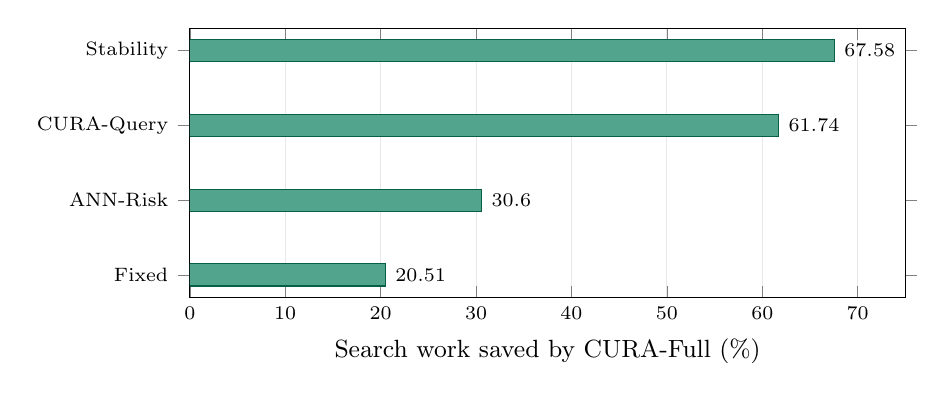
\begin{tikzpicture}
\begin{axis}[width=0.88\columnwidth,height=5.0cm,xbar,bar width=8pt,xlabel={Search work saved by CURA-Full (\%)},symbolic y coords={Fixed,ANN-Risk,CURA-Query,Stability},ytick=data,xmin=0,xmax=75,xmajorgrids=true,grid style={gray!18},axis line style={black},tick label style={font=\scriptsize,text=black},label style={font=\small,text=black},nodes near coords,every node near coord/.append style={font=\scriptsize,text=black,anchor=west}]
\addplot[fill=CuraGreen!70,draw=CuraDark] coordinates {(20.51,Fixed) (30.60,ANN-Risk) (61.74,CURA-Query) (67.58,Stability)};
\end{axis}
\end{tikzpicture}
\caption{\textbf{Ablation summary.} Percentage reduction in realized search work achieved by \cura{}-Full relative to each deployable comparator.}
\label{fig:ablation}
\end{figure}

% ======================================================================
% 8 ANN VS IR
% ======================================================================
\section{Why ANN Recall Is Not the Final Objective}
\label{sec:annvsir}
A striking result is that \cura{}-Full has an ANN violation rate of $10.0\%$, which is greater than the fixed baseline's $3.5\%$. Yet \cura{}'s downstream violation rate is only $1.0\%$.

This is not a contradiction. It is the trade-off \cura{} is explicitly designed to exploit. The controller permits exact-neighbor misses when those misses do not cause material downstream ranking degradation.

The IR oracle demonstrates the distinction even more clearly. Within the tested budget grid it permits $29\%$ ANN-target violations while producing $0\%$ downstream IR violations. Therefore maximizing exact ANN Recall@10 is stricter than necessary for some queries.

% ======================================================================
% 9 CALIBRATION
% ======================================================================
\section{Risk Calibration}
\label{sec:calibration}
Because the controller operates on predicted risk, probability quality is central to the method.

\begin{table}[!t]
\centering
\caption{Risk-prediction quality. Lower Brier and ECE are better; higher ROC-AUC is better.}
\label{tab:calibration}
\resizebox{\columnwidth}{!}{%
\begin{tabular}{llrrr}
\toprule
Split & Model & Brier & ECE & ROC-AUC \\
\midrule
MS MARCO & CURA-Query & 0.01462 & 0.01831 & 0.8243 \\
MS MARCO & \textbf{CURA-Full} & \textbf{0.01245} & \textbf{0.01481} & \textbf{0.9290} \\
TREC OOD & CURA-Query & 0.03068 & 0.00129 & 0.8125 \\
TREC OOD & \textbf{CURA-Full} & \textbf{0.02708} & 0.00802 & \textbf{0.8574} \\
\bottomrule
\end{tabular}%
}
\end{table}

On held-out MS MARCO, adding partial-search features raises ROC-AUC from $0.8243$ to $0.9290$. This provides independent evidence that search-state information is useful beyond query features alone.

% ======================================================================
% 10 OOD
% ======================================================================
\section{Out-of-Distribution Evaluation}
\label{sec:ood}
All TREC-DL-2019 queries are excluded from model fitting and probability calibration. The oracle ANN-versus-IR budget gap becomes substantially weaker on this deeply judged set. This is an important negative result because it indicates that the amount of downstream-safe ANN savings depends on the evaluation regime.

On 43 TREC-DL-2019 queries CURA-Full records an \emph{observed} 2.33\% IR violation rate versus 0\% under fixed HNSW, and 2384.58 versus 2721.88 computations per query (12.39\% less work). Its OOD ROC-AUC is 0.8574 and ECE approximately 0.0080. These are query-shift results on the MS MARCO passage domain, not independent-domain transfer or a formal 5\% guarantee.

% ======================================================================
% 11 MANUAL ERROR TAXONOMY
% ======================================================================
\section{Financial-Domain Experiment: BEIR FiQA}
\label{sec:fiqa}
A separate budget sweep uses BEIR FiQA with 57,638 documents and 648 queries. For an exploratory within-FiQA controller, 388 queries are used for fitting, 129 for calibration and 131 for local held-out comparison. Because these are drawn from the benchmark's published test queries, the numbers are not untouched official BEIR test results. This simplified controller uses query text and an \ef$=10$ probe's work/latency, not the full MS MARCO score-gap features. It is \emph{not} zero-shot MS MARCO-to-FiQA transfer.

\begin{table*}[!t]
\centering
\caption{\textbf{FiQA local held-out results (131 queries).} Realized work counts repeat-search overhead. The controller is fitted separately on FiQA.}
\label{tab:fiqa}
\resizebox{0.93\textwidth}{!}{%
\begin{tabular}{lrrrrrr}
\toprule
Method & Mean \ef{} & IR violations & Mean \ndcg{} & Work/query & Mean latency (ms) & Wilson 95\% upper bound\\
\midrule
Fixed HNSW & 32.00 & 3.05\% & 0.22014 & \textbf{1097.08} & \textbf{0.21490} & 7.59\%\\
Simplified CURA-FiQA & 47.74 & 3.05\% & 0.21787 & 1922.87 & 0.38564 & 7.59\%\\
\bottomrule
\end{tabular}%
}
\end{table*}

\paragraph{Negative result.} The separately fitted controller uses \textbf{75.27\% more realized work} at the same observed violation rate as the calibration-selected fixed \ef$=32$ policy. Both methods fail on 2 common queries; 2 additional queries fail only under fixed search and 2 only under simplified CURA. The observed violation rate is 4/131 for both, with a Wilson 95\% upper bound of 7.59\%, \emph{above} the nominal 5\% target. Thus neither method establishes a held-out risk guarantee.

\paragraph{Overhead diagnosis.} The probe contributes about 451.32 computations per query, 112/131 queries require a second search, and 51/131 receive budgets greater than the fixed \ef$=32$. Feature weakness, conservative calibration and repeated graph traversal are plausible but not causally isolated explanations. The evaluated held-out split is kept frozen.


\section{Failure Evidence and Manual-Review Status}
\label{sec:manual}
The earlier MS MARCO 50-case diagnostic table contains only three actual downstream violations, so it does \emph{not} establish a human-reviewed taxonomy of 50 genuine CURA policy failures.

In FiQA, 65 distinct queries exhibit an IR-unsafe outcome under fixed HNSW at \ef$=10$. We prepare a separate 50-query review worksheet, each case including relevant passages, exact-search passages, approximate top-ranked passages and the measured nDCG loss. All 50 reconstructed results match previously saved scores. Of these selected cases, 44 have HNSW nDCG@10 equal to zero and six have degraded but nonzero nDCG@10.

\begin{table}[!t]
\centering
\caption{\textbf{Evidence preparation, not a completed human taxonomy.} All failures refer to fixed HNSW \ef$=10$, not deployed CURA.}
\label{tab:fiqa_manual}
\begin{tabular}{lr}
\toprule
Case status & Count\\
\midrule
Distinct failing queries available & 65\\
Cases selected for review & 50\\
Reconstruction checks passed & 50\\
Zero approximate nDCG@10 & 44\\
Degraded but nonzero nDCG@10 & 6\\
Human reviews completed in latest audit & 1\\
Human reviews remaining & 49\\
\bottomrule
\end{tabular}
\end{table}

The existing assistant-prepared notes are evidence \emph{drafts}, not verified human judgments. A reviewer must inspect the actual passages, confirm or change the failure category and document supporting IDs/ranks and a plausible remedy. The full 50-case human-reviewed taxonomy remains pending before the final course submission.


\section{Discussion}
\label{sec:discussion}
\subsection{What Did the Project Establish?}
The initial research question was whether different queries require different ANN budgets. The results support a more precise conclusion:
\begin{quote}
\textbf{On the controlled MS MARCO queries, adaptive budgets can reduce computation for an observed downstream-risk tolerance; that benefit need not transfer to a separately fitted controller or another domain.}
\end{quote}
This formulation is stronger than merely predicting query difficulty because it connects search effort directly to an application-level quality constraint.

\subsection{Why Query-Only Allocation Is Insufficient}
The query-only variant is extremely conservative. It achieves no observed downstream violations but requires $7130.76$ distance computations per query. The full model reduces this to $2727.97$. Thus the state of the actual search process is much more informative than query semantics alone.

\subsection{Why Mean ef Is Not Enough}
ANN-Risk chooses a lower mean \ef{} than fixed search: $84.46<96$. Nevertheless, ANN-Risk performs more total realized work: $3930.62>3431.77$. The reason is adaptive decision overhead. This demonstrates why a systems evaluation based only on selected \ef{} would be misleading.

\subsection{Interpreting the FiQA Negative Result}
Our simpler FiQA controller is slower than fixed HNSW, underscoring the importance of informative partial-search features and avoiding a second graph search after the probe. Continuation-based search that reuses its frontier remains future work, not a measured gain.

\subsection{Remaining Oracle Headroom}
The IR oracle requires $779.835$ mean distance computations, while \cura{}-Full requires $2727.965$. The difference is approximately $1948.13$ distance computations per query. Therefore the controller captures meaningful efficiency but still leaves substantial downstream-safe headroom for improved risk estimation and single-pass early termination.

% ======================================================================
% 13 LIMITATIONS
% ======================================================================
\section{Limitations and Claim Boundaries}
\label{sec:limitations}
\begin{tcolorbox}[colback=RiskLight,colframe=RiskRed,title=\textbf{Claims Not Made},fonttitle=\small,boxrule=0.8pt]
\small
\begin{itemize}
\item We do not report the controlled subset as official full-corpus MS MARCO effectiveness.
\item We do not claim that ANN recall is unimportant.
\item We do not claim that every query has a smaller IR-safe than ANN-safe budget.
\item ANN-Risk is not an official DARTH reproduction.
\item Patience-Inspired is not an official Patience reproduction.
\item The current evidence does not establish universal cross-domain generalization or a formal 5\% risk guarantee.
\item FiQA uses a separately fitted reduced-feature controller and reuses official test queries for development.
\item The 50 fixed-budget FiQA failures are not yet fully human-reviewed.
\end{itemize}
\end{tcolorbox}

\paragraph{Controlled corpus.}
The final primary experiment uses approximately one million passages rather than the complete 8.8M MS MARCO collection.

\paragraph{Index family.}
The learned controller is evaluated only with HNSW. IVF-style indexes and other iterative ANN methods remain future work.

\paragraph{Encoder.}
The primary experiments use one fixed MiniLM-based encoder. Different embedding geometries may change query hardness and calibration.

\paragraph{Domain evidence and benchmark limitations.}
Our experiments now include a BEIR FiQA financial-domain collection, but the controller fit reuses official FiQA test queries as development data and therefore is not official untouched benchmark evaluation. The simplified FiQA controller yields a negative efficiency result rather than positive cross-domain replication.

\paragraph{Calibration and reproduction.}
Reusing the same calibration set for probability fitting and policy selection limits coverage interpretation. Although result tables and code are committed, a full clean-environment rerun from downloaded data and rebuilt embeddings/indexes has not yet been independently verified.

\paragraph{Recent baseline implementations.}
Patience and DARTH are highly relevant recent systems, but the experiments here do not reproduce their official implementations. A definitive systems comparison should run the original code under the same corpus, encoder, risk constraint, and cost accounting.

\paragraph{OOD sample size.}
TREC-DL-2019 contains only 43 deeply judged queries. The OOD result is therefore informative but statistically limited.

% ======================================================================
% 14 CONCLUSION
% ======================================================================
\section{Conclusion}
\label{sec:conclusion}
This work studies query-specific ANN search-budget allocation from the perspective of downstream retrieval quality. Oracle experiments first show that the search effort required to preserve exact ANN neighbors and the effort required to preserve downstream ranking quality can differ substantially.

We then introduce \cura{}, a calibrated utility-risk controller that predicts the probability that a candidate HNSW budget will cause unacceptable nDCG@10 degradation.

On held-out million-scale MS MARCO, \cura{}-Full:
\begin{itemize}
\item maintains only \textbf{1.0\% downstream violations} under a \textbf{5\% risk SLA};
\item reduces realized search work by \textbf{20.5\% relative to fixed HNSW};
\item reduces work by \textbf{30.6\% relative to ANN-risk adaptation};
\item uses \textbf{61.7\% less work than query-only CURA};
\item uses \textbf{67.6\% less realized work than the Patience-inspired stability baseline};
\item records 2.33\% observed violations and 12.39\% lower work on the 43-query TREC-DL-2019 query-shift set.
\end{itemize}

The separately fitted reduced-feature FiQA controller instead requires \textbf{75.27\% more} work than fixed HNSW for the same observed violation rate. We therefore conclude that preserving downstream utility is distinct from exact-neighbor recovery, but success of practical adaptive policies depends on domain, features and probe overhead.

\begin{tcolorbox}[colback=CuraLight,colframe=CuraGreen,boxrule=0.8pt,arc=3pt,left=5pt,right=5pt,top=4pt,bottom=4pt]
\centering\small
\textbf{Future direction: adaptive ANN computation under calibrated downstream-risk constraints across multiple index families, encoders, and retrieval domains.}
\end{tcolorbox}

% ======================================================================
% APPENDIX
% ======================================================================
\appendix
\section{Alignment with the Assigned Project}
The final implementation maps directly onto the central dimensions of the query-specific ANN budgeting project.

\begin{table*}[!t]
\centering
\caption{Alignment between the assigned research problem and the completed experimental design.}
\resizebox{0.96\textwidth}{!}{%
\begin{tabular}{lll}
\toprule
\textbf{Project dimension} & \textbf{Implementation in this work} & \textbf{Evidence} \\
\midrule
Per-query ANN effort & CURA selects HNSW \ef{} per query & Mean selected ef = 51.97 on held-out test \\
Cheap decision features & Query + inexpensive partial HNSW probe & Query-only vs full ablation \\
Calibrated policy & Isotonic probability calibration & Brier, ECE, ROC-AUC reported \\
Target constraint & Downstream nDCG-loss risk SLA & 1.0\% observed violation under 5\% target \\
Distribution shift & TREC-DL-2019 held out completely & OOD calibration and violations reported \\
ANN effectiveness & ANN Recall@10 & ANN violation rates reported \\
End-to-end IR effectiveness & nDCG@10, Recall@100, MRR@10 & Exact and ANN retrieval evaluated \\
Efficiency & Distance computations + latency & Mean and p95 measurements \\
Query features ablation & CURA-Query & 7130.76 realized work \\
Partial-search ablation & CURA-Full & 2727.97 realized work \\
Classical system baseline & Fixed HNSW & 3431.77 realized work \\
Adaptive ANN baseline & ANN-Risk & 3930.62 realized work \\
Early-exit baseline & Patience-inspired stability & 8413.95 realized work \\
Statistics & Bootstrap + paired randomization & 95\% CIs and query-level $p$ values \\
Manual case preparation & 50 low-budget FiQA failures & 1/50 independently reviewed \\
Reproducibility & Scripts and saved artifacts & Fresh full rerun pending \\
\bottomrule
\end{tabular}%
}
\end{table*}

\section{Reproducibility Checklist}
\begin{table}[!t]
\centering
\resizebox{\columnwidth}{!}{%
\begin{tabular}{ll}
\toprule
Item & Status \\
\midrule
Random seed & 42 \\
Corpus size recorded & Yes \\
Query split saved & Yes \\
Encoder version recorded & Yes \\
HNSW parameters recorded & Yes \\
Candidate budgets recorded & Yes \\
ANN target recorded & Yes \\
IR loss tolerance recorded & Yes \\
Calibration protocol recorded & Yes \\
Probe cost included & Yes \\
Repeated-search cost included & Yes \\
Exact reference cached & Yes \\
Bootstrap confidence intervals & Yes \\
Paired randomization tests & Yes \\
Manual 50-case human review & 1/50 pending \\
OOD evaluation & Yes \\
Official DARTH reproduction & No \\
Official Patience reproduction & No \\
Full 8.8M run & No \\
\bottomrule
\end{tabular}%
}
\end{table}

\section{Generative-AI Assistance Statement}
Generative-AI tools helped with code drafting and debugging, experiment organization, literature navigation, document editing, and preliminary failure-analysis notes. Numerical results are transcribed from recorded experimental output rather than generated by the assistant; writing this manuscript did not run new training. AI-prepared case notes must not be reported as independent human judgments. The author is responsible for verifying the final experimental claims, compliance and bibliography.

% ======================================================================
% REFERENCES
% ======================================================================
\begin{thebibliography}{99}

\bibitem{malkov2020hnsw}
Yury A. Malkov and Dmitry A. Yashunin.
\newblock Efficient and robust approximate nearest neighbor search using hierarchical navigable small world graphs.
\newblock \emph{IEEE Transactions on Pattern Analysis and Machine Intelligence}, 42(4):824--836, 2020.

\bibitem{johnson2017faiss}
Jeff Johnson, Matthijs Douze, and Herv\'e J\'egou.
\newblock Billion-scale similarity search with GPUs.
\newblock arXiv:1702.08734, 2017.

\bibitem{bajaj2016msmarco}
Payal Bajaj, Daniel Campos, Nick Craswell, Li Deng, Jianfeng Gao, Xiaodong Liu, Rangan Majumder, Andrew McNamara, Bhaskar Mitra, Tri Nguyen, Mir Rosenberg, Xia Song, Alina Stoica, Saurabh Tiwary, and Tong Wang.
\newblock MS MARCO: A human generated machine reading comprehension dataset.
\newblock arXiv:1611.09268, 2016.

\bibitem{craswell2020trecdl}
Nick Craswell, Bhaskar Mitra, Emine Yilmaz, Daniel Campos, and Ellen M. Voorhees.
\newblock Overview of the TREC 2019 Deep Learning Track.
\newblock In \emph{Text REtrieval Conference (TREC)}, 2020.

\bibitem{jarvelin2002cg}
Kalervo J\"arvelin and Jaana Kek\"al\"ainen.
\newblock Cumulated gain-based evaluation of IR techniques.
\newblock \emph{ACM Transactions on Information Systems}, 20(4):422--446, 2002.

\bibitem{reimers2019sbert}
Nils Reimers and Iryna Gurevych.
\newblock Sentence-BERT: Sentence embeddings using Siamese BERT-networks.
\newblock In \emph{Proceedings of EMNLP-IJCNLP}, pages 3982--3992, 2019.

\bibitem{aumuller2020ann}
Martin Aum\"uller, Erik Bernhardsson, and Alexander Faithfull.
\newblock ANN-Benchmarks: A benchmarking tool for approximate nearest neighbor algorithms.
\newblock \emph{Information Systems}, 87:101374, 2020.

\bibitem{subramanya2019diskann}
Suhas Jayaram Subramanya, Fnu Devvrit, Harsha Vardhan Simhadri, Ravishankar Krishnawamy, and Rohan Kadekodi.
\newblock DiskANN: Fast accurate billion-point nearest neighbor search on a single node.
\newblock In \emph{Advances in Neural Information Processing Systems}, 2019.

\bibitem{guo2020scann}
Ruiqi Guo, Philip Sun, Erik Lindgren, Quan Geng, David Simcha, Felix Chern, and Sanjiv Kumar.
\newblock Accelerating large-scale inference with anisotropic vector quantization.
\newblock In \emph{Proceedings of the 37th International Conference on Machine Learning}, pages 3887--3896, 2020.

\bibitem{kulkarni2023ladr}
Hrishikesh Kulkarni, Sean MacAvaney, Nazli Goharian, and Ophir Frieder.
\newblock Lexically-Accelerated Dense Retrieval.
\newblock In \emph{Proceedings of the 46th International ACM SIGIR Conference on Research and Development in Information Retrieval}, pages 152--162, 2023.

\bibitem{zhang2023hybrid}
Peitian Zhang, Zheng Liu, Shitao Xiao, Zhicheng Dou, and Jing Yao.
\newblock Hybrid Inverted Index Is a Robust Accelerator for Dense Retrieval.
\newblock In \emph{Proceedings of the 2023 Conference on Empirical Methods in Natural Language Processing}, pages 1877--1888, 2023.

\bibitem{busolin2024early}
Francesco Busolin, Claudio Lucchese, Franco Maria Nardini, Salvatore Orlando, Raffaele Perego, and Salvatore Trani.
\newblock Early Exit Strategies for Approximate $k$-NN Search in Dense Retrieval.
\newblock In \emph{Proceedings of the 33rd ACM International Conference on Information and Knowledge Management}, pages 3647--3652, 2024.

\bibitem{teofili2025patience}
Tommaso Teofili and Jimmy Lin.
\newblock Patience in Proximity: A Simple Early Termination Strategy for HNSW Graph Traversal in Approximate $k$-Nearest Neighbor Search.
\newblock In \emph{Advances in Information Retrieval -- ECIR 2025}, LNCS 15574, pages 401--407, Springer, 2025.

\bibitem{zhang2026adaptive}
Chao Zhang and Ren\'ee J. Miller.
\newblock Distribution-Aware Exploration for Adaptive HNSW Search.
\newblock \emph{Proceedings of the ACM on Management of Data}, 2026.

\bibitem{chatzakis2026darth}
Manos Chatzakis, Yannis Papakonstantinou, and Themis Palpanas.
\newblock DARTH: Declarative Recall Through Early Termination for Approximate Nearest Neighbor Search.
\newblock In \emph{ACM SIGMOD International Conference on Management of Data}, 2026.

\bibitem{lu2026terminus}
Jianan Lu, Asaf Cidon, and Michael Freedman.
\newblock When Enough Is Enough: Rank-Aware Early Termination for Vector Search.
\newblock In \emph{Proceedings of Machine Learning and Systems}, volume 8, 2026.

\bibitem{guo2017calibration}
Chuan Guo, Geoff Pleiss, Yu Sun, and Kilian Q. Weinberger.
\newblock On Calibration of Modern Neural Networks.
\newblock In \emph{Proceedings of the 34th International Conference on Machine Learning}, pages 1321--1330, 2017.

\end{thebibliography}
\end{document}